\documentclass[conference,compsoc]{IEEEtran}

\usepackage{graphicx}
\usepackage[utf8]{inputenc}
\usepackage[T1]{fontenc}
\usepackage{xcolor,graphicx}
\usepackage{ragged2e}
\usepackage[top=0.6in,bottom=0.6in,right=1in,left=1in]{geometry}

\begin{document}

\title{Final Year Project}
% author names
\author{\IEEEauthorblockN{Sammar Tahir}{Arkadiusz Mamala}\\{Usman Sattar}\\
\IEEEauthorblockA{\textsc{Galway Mayo Institute of Technology\\Applied Project \& Minor Dissertation}}}
\maketitle

\textbf{GitHub}
\\
https://github.com/ArekMamala/FinalYearProject

\section{Introduction}
For our project we wanted to make a wearable wristband that allows a user to keep track of how many punches hit an object, tracking the speed of movement and calculating the beats per minute whilst continuously punching . We also want to connect the wristband to a laptop/phone so the user is able to get all his information tracked and displayed in an elegant and sleek app.
\\
\textbf{Reason for Choosing Project:}

The reasons that we decided to develop this application is because we find this idea very interesting. Sports is a topic that we are all involved in inside of college and out. We came up with this idea when we were at a boxing class when we couldn't decide who had more power. It’s a project that we feel will challenge us in developing it and get it working the way we have designed it.
\\
\textbf{The technologies we plan on using are:}
\begin{itemize}
\item{Web servers to store our data (AWS)}
\item{Wearable tracker}
\item{Angular}
\item{Javascript/C+}
\item{Google Drive}
\end{itemize}
\subsection*{Architecture}

The application on the phone is going to work with user control. The application is going to count punches, update data sheet, calculate the BPM of user while punching. This app is going to be an alternative to the research of the wearable device.
\\
\textbf{User will have three options within the application:}
\begin{itemize}
\item Calculate the number of punches against time.
\item Calculate the number of punches and beats per minute against time.
\item Open data log sheet to view their history. To view their progression.
\end{itemize}

\subsection*{Work Allocation}
We are allocating this project into three sections.
\textbf{First Step:}

Firstly we are going to start our research. We are going to deeply research in how this wearable device is going to work and what it takes to develop this new piece of technology. We need to understand what language is going to be used in constructing this. We need to know what sensors are required and how all data is going to be recorded.
\\
\textbf{Second Step:}

During the term our research is going to be a piece of document in how this wearable device can be achieved and possible drawing and animations of how it may work. But to back up our research, we need a physical piece that we can show and present. So we as a group decided to construct an application that is downloadable on mobile phone. This phone application is an alternative to the wearable device. The application is going to record the number of punches. The application is going to record and store data. For example is it going to store the number of punches under a certain amount of time.
\\
\textbf{Third Step:}

Whilst two members of the team are constructing the application. One person is going to specifically manage the database. They will have the responsibility to create the AWS account and link it up to the database. Overall, they are responsible for the whole database section of this project and to link it up to the application, that is works efficiently.

\section{Research}

\subsection*{Artificial Neural Network}
In the oxford dictionary it says, “artificial intelligence is an area of study concerned with making computers copy intelligent human behaviour \cite{knowles2006oxford}.” If you google the question that I just asked, you’ll get something like “the theory and development of computer systems able to perform tasks normally requiring human intelligence, such as visual perception, speech recognition, decision-making, and translation between languages.”

To really understand what Artificial intelligence (AI) is, we first must know what Intelligence is. When people talk about intelligence, they identify it with “the ability to solve hard problems.” Some people say it’s “Maybe it is too early
to define intelligence. It is obvious that, after decades of study, we still do not know very much about it. There are more questions than answers \cite{wang2007logic}.” This is where we stumble upon the idea of Artificial Intelligence.
\\
\textbf{The birth of the idea}

The birth of AI is bizarre from what normal people would think. AI wasn’t made along with computers it was sort of this fictional monster. The first AI possibly made was by Mary Shelly when she wrote Frankenstein in 1818 \cite{shelley2012frankenstein}.So technically the first ever AI was made long before we even thought of the idea. The main concept that comes into people’s minds is something man made that is designed to solve all our lives biggest questions. \cite{bostrom2014ethics}

For this project we have to learn how to build a neural database. To build the actual neural network we are using a program called Keras which comes with Anaconda, a powerful tool used with Python. We look at different approaches when it comes to training a system. For example, taking this project in hand, we need to train the system to recognize the different types of punches thrown. Before learning out neural networks we would need to know what a neuron is.\\
\textbf{Neuron}

\textit{"A specialized cell transmitting nerve impulses; a nerve cell."} \\ A neuron has an input($x$) and output($y$). The input normally has a weight to it and a bias($b$) with is usually This image below will show you how a neuron looks.

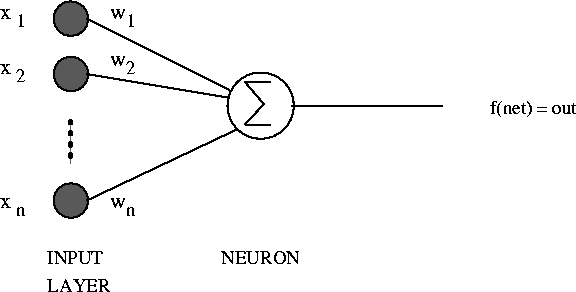
\includegraphics[scale=.4]{Neuron.png}
Neural networks are a set of algorithms, modeled loosely after the human brain, that are designed to recognize patterns. Neural networks are being applied to many real-life problems today, including speech and image recognition, spam email filtering, finance, and medical diagnosis, to name a few.

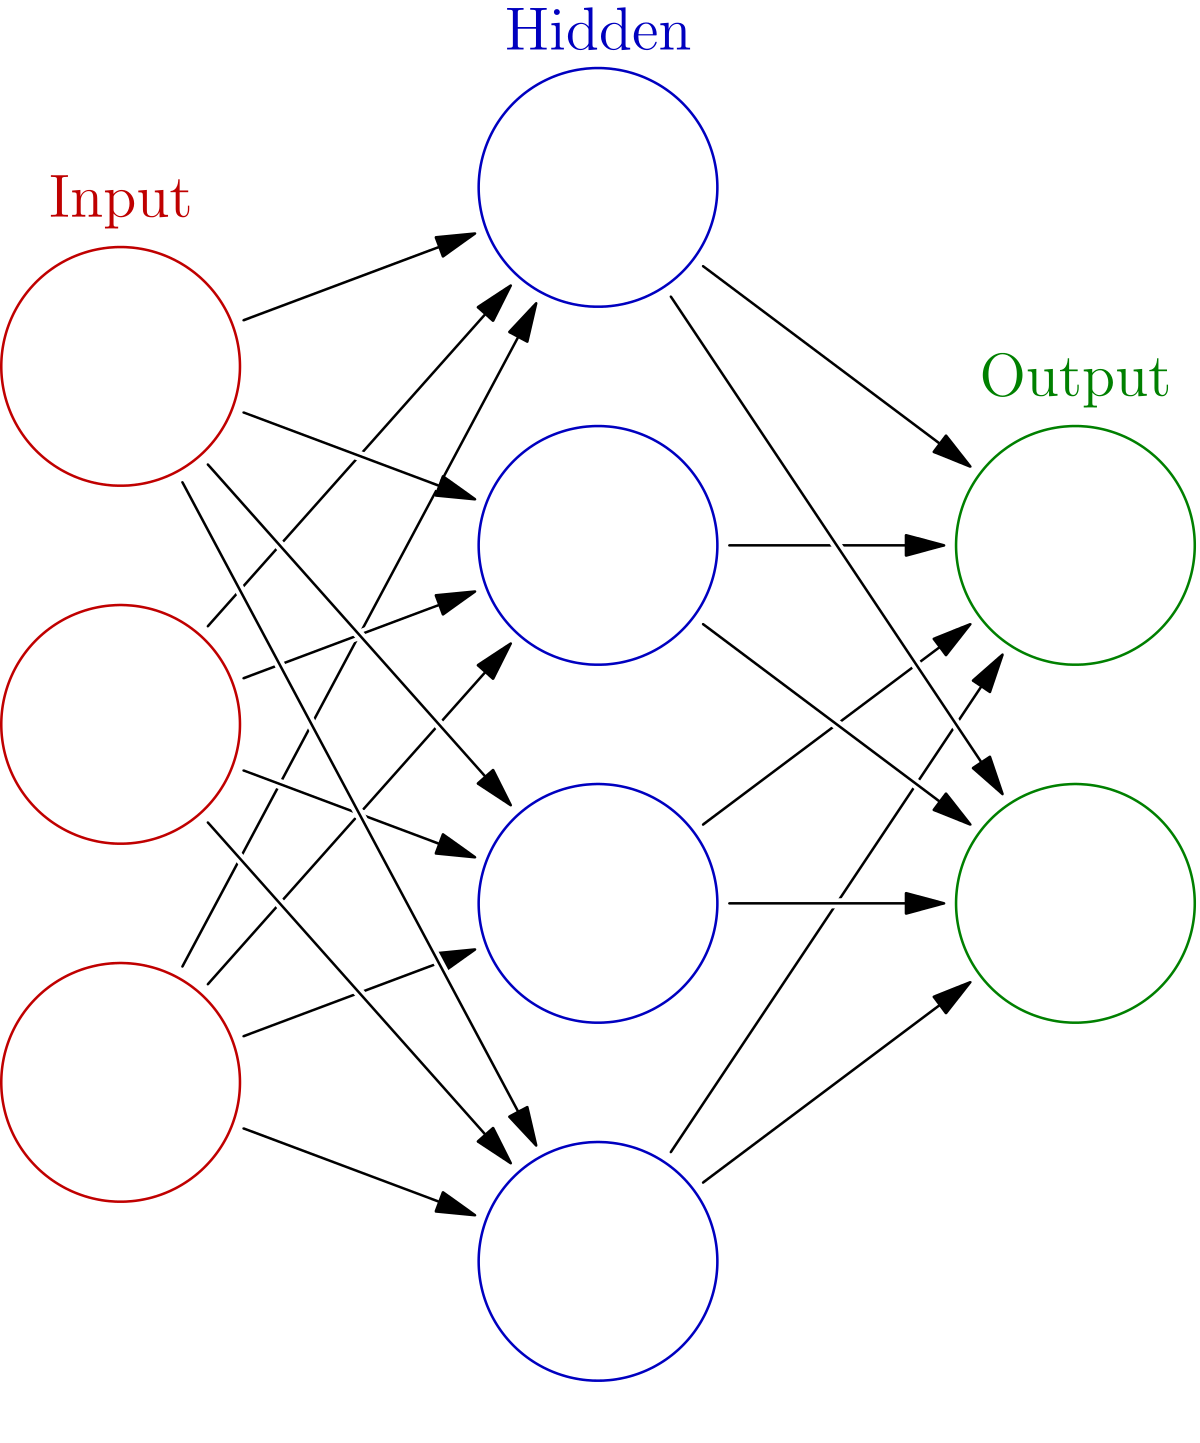
\includegraphics[scale=.19]{NeuralNetwork.png}
\textbf{3 reasons to study neural computation:}\\
\textbf{1.} To understand how the brain actually works: it's very large and very complicated and made from things that die when you poke it, so we need to use computer simulations.\\
\textbf{2.} To grasp a neuron-inspired model of parallel computation and their adaptive connections: it is a very different style from sequential computation.\\
\textbf{3.} To solve practical problems by using novel learning algorithms inspired by the brain: learning algorithms can be very useful even if they are not how the brain actually works.
\\
With these tools, we can train the model to recognize the type of punches:\\
\textit{Jab\\hook\\Uppercut}

Using tensorflow with python to do this project. Tensorflow is a symbolic math library which can be used for machine learning. Keras is used to make the neural network. Numpy and pyplot is used to plot the data. Before making the data set for machine learning we'd need to learn of the core core concepts of making data-sets. This is how to shape your data and how to get it ready for training. To understand the layout of data-sets I used some examples online and decided to use the well know the iris data-set. This data-set collects data points from a hundred and fifty different samples of flower. It uses the petal length/width and the sepal length/width and sorts them into three types of iris.
\begin{verbatim}
from sklearn.datasets import load_iris

iris = load_iris()
iris

'data': array([[5.1, 3.5, 1.4, 0.2],
               [4.9, 3. , 1.4, 0.2],
               [4.7, 3.2, 1.3, 0.2],
               [4.6, 3.1, 1.5, 0.2],
\end{verbatim}
I wanted to do something similar to this using the x,y,z axis on the device and the accelerometer and sorting them into the three types of punches the device would register. I've learnt that by training a neural network with these values and telling it the type of punch it is I can then build a neural network than can reference from new values what type of punch is thrown. The dataset that I'm going to make will contain four values and the type of punch it should be. The punch will be classified as 0, 1 or 2.

\section*{How is physics applied to boxing}
Physics occurs in punching because of energy. Person uses energy in order for a punch to be carried out. That is why, as well as energy we need momentum, work, power, and velocity. Before a boxer punches, he has potential energy which is stored energy. Once, the boxer begins to punch potential energy turns into kinetic energy.

Boxing is more than the brutal beating up of one another; it is a sport that applies many physics laws. If a fighter uses physics correctly, he will likely get the victory; but if he does not, he will probably lose.

As soon as a boxer starts to move his or her shoulders and arms and eventually the fists, his/her potential energy is being converted into kinetic energy.\\
\textbf{Kinetic energy is calculated by using the formula:}

$Kinetic Energy = (1/2)mv^2$

The fist has its maximum velocity when it hits something. The collision then causes the fist to slow down, eventually the fighter begins applying a force to retract his/her arm.\\
\textbf{This speed is calculated using:}

$Velocity = Distance / Time$
\\
What is Velocity? The speed of something in a given direction.

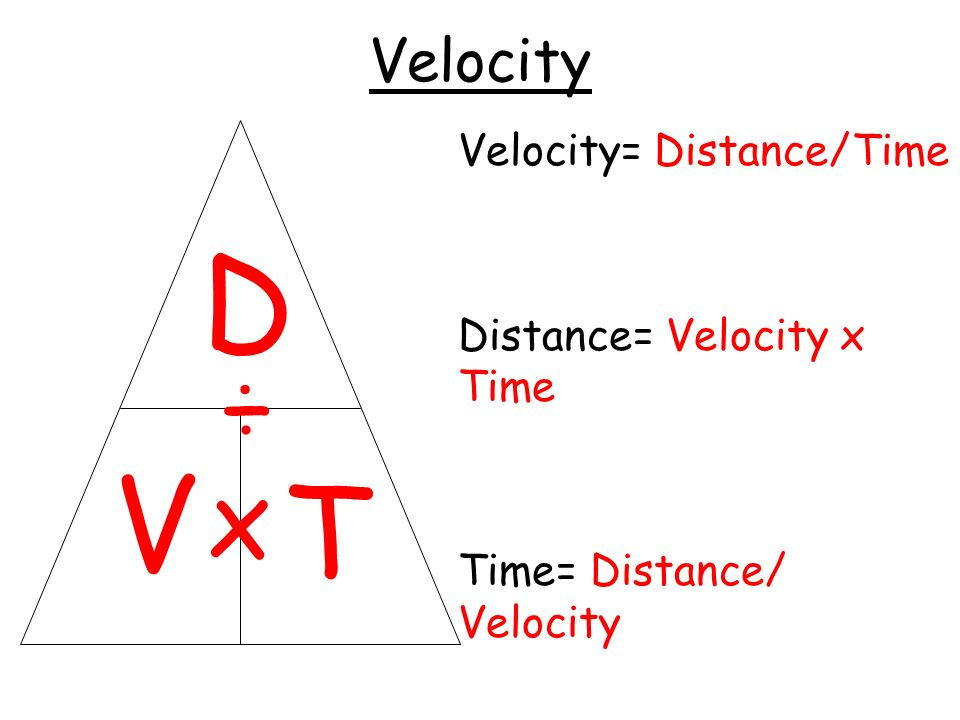
\includegraphics[scale=.3]{Velocity.jpeg}



% references section
\bibliographystyle{plain}
\bibliography{refs} % 


\end{document}
